\documentclass[12pt]{spieman}  % 12pt font required by SPIE;
%\documentclass[a4paper,12pt]{spieman}  % use this instead for A4 paper
\usepackage{amsmath,amsfonts,amssymb}
\usepackage{graphicx}
\usepackage{setspace}
\usepackage{tocloft}
\usepackage{hyperref}
\usepackage{graphicx}
\usepackage{float}
\usepackage{wrapfig}
\title{Information Retrieval - Submission Report \\Project N.14: Art For Sale}

\author{Jeferson Morales Mariciano}
\author{Filippo Piloni}
\affil{Università della Svizzera italiana, Faculty of Informatics, Lugano, Switzerland}

\renewcommand{\cftdotsep}{\cftnodots}
\cftpagenumbersoff{figure}
\cftpagenumbersoff{table} 
\begin{document}

\begin{wrapfigure}{l}{0.25\textwidth}
    
\includegraphics[width=0.25\textwidth, trim={0cm 0cm 0cm 7cm}]{USI_logo.png}
\end{wrapfigure}

\maketitle
\tableofcontents
\newpage

\begin{spacing}{1}   % use double spacing for rest of manuscript

    \section{Introduction}
    The Information Retrieval course project \textit{"ArtForSale"} aims to be a working prototype of an information
    retrieval system for a specific task: to display for-sale artworks from art selling related websites
    listed in Section \ref{sec:websites}.
    The system has around $\approx 8,500$ indexed documents for searching, browsing and presented through a
    user-friendly and intuitive interface, further details in UI/UX Section \ref{sec:ui}, \ref{sec:ux}.

    \subsection{Websites}\label{sec:websites}
    The following websites were chosen for the project based on availability of data, ease of scraping and
    low restrictions regarding policies and terms of use to scrape documents i.e. \textit{robots.txt} rules:

    \begin{itemize}
        \item \url{www.artsy.net}
        \item \url{www.artfinder.com}
        \item \url{www.saatchiart.com}
    \end{itemize}

    The cumulative number of documents gathered from the above websites is around $\approx 8,500$ stored in
    \textit{results.json} file containing the list of samples in JSON format.
    Further information concerning the scraping process and implementation is discussed
    in Crawler Section \ref{sec:crawling}.

    \subsection{Features}
    The course project requires 2 additional categorized features to be implemented besides the retrieval system:
    1 each from simple and complex group features.\\
    The \textit{Art For Sale} project implements 2 + 1 bonus additional simple features:

    \begin{itemize}
        \item Simple
              \begin{itemize}
                  \item \textbf{Result presentation}:
                        results should be presented in a tabular format so that many results could be seen at the same time.
                        Each table cell should contain appropriate information for your project.
                  \item \textbf{Filtering}:
                        in addition to being able to search by title, an user should be able to filter the
                        results based on at least 3 relevant attributes for your project.
              \end{itemize}

        \item Complex
              \begin{itemize}
                  \item \textbf{Automatic recommendation}:
                        In addition to the relevant search results pertaining to the user query,
                        the user should also be suggested "similar" products based on, say, category, description,
                        price etc. The ordering among the recommended items is not important.
                        However, you should mention how did you arrive at the recommendations.
                        For this purpose, you can use any open-source recommenders available.
              \end{itemize}
    \end{itemize}

    Shown results are sorted in descending order of relevance from left to right in the tabular view.\\
    Implementation details of features are on Architecture Section \ref{sec:architecture}.\\
    Moreover, by exploiting the automatic recommandation feature implemented using category tags
    and the filtering feature to filter them,
    the \textbf{Results clustering} complex feature was tackled by allowing to
    group the results into topics based on category tags.
    Though, a negative filter to exclude documents based on categories was not added,
    thus partially implementing another extra feature.\\

    %%%%%%%%%%%%%%%%%%%%%%%%%%%%%%%%%%%%%%%%%%%%%%%%%%%%%%%%%%%%%%%%%
    \section{Architecture}\label{sec:architecture}

    The \textbf{Information Retrieval System} has capabilities limited to a
    \textbf{TIS} \footnote{Text Information System}
    with \textbf{Text retrieval}.\\
    The \textbf{Text Access} part helping users to retrieve the right information at the right time,
    is structured by connecting the system with users in both modes:
    \begin{itemize}
        \item \textbf{Pull}: user takes initiative to fetch ad-hoc relevant information from the system,
              which offers \textbf{querying} and \textbf{browsing} capabilities.
              Satisfies \textbf{short-term needs}.
        \item \textbf{Push}: system takes initiative and has good knowledge of what are the user's
              \textbf{long-term needs} of information throughout the filtering and recommendation system
              using \textbf{browsing traces} to model the behavior of the user.
    \end{itemize}

    \begin{figure}[H]
        \centering
        \caption{Search Engine Architecture of \textit{ArtForSale} project}
        \label{fig:architecture}
        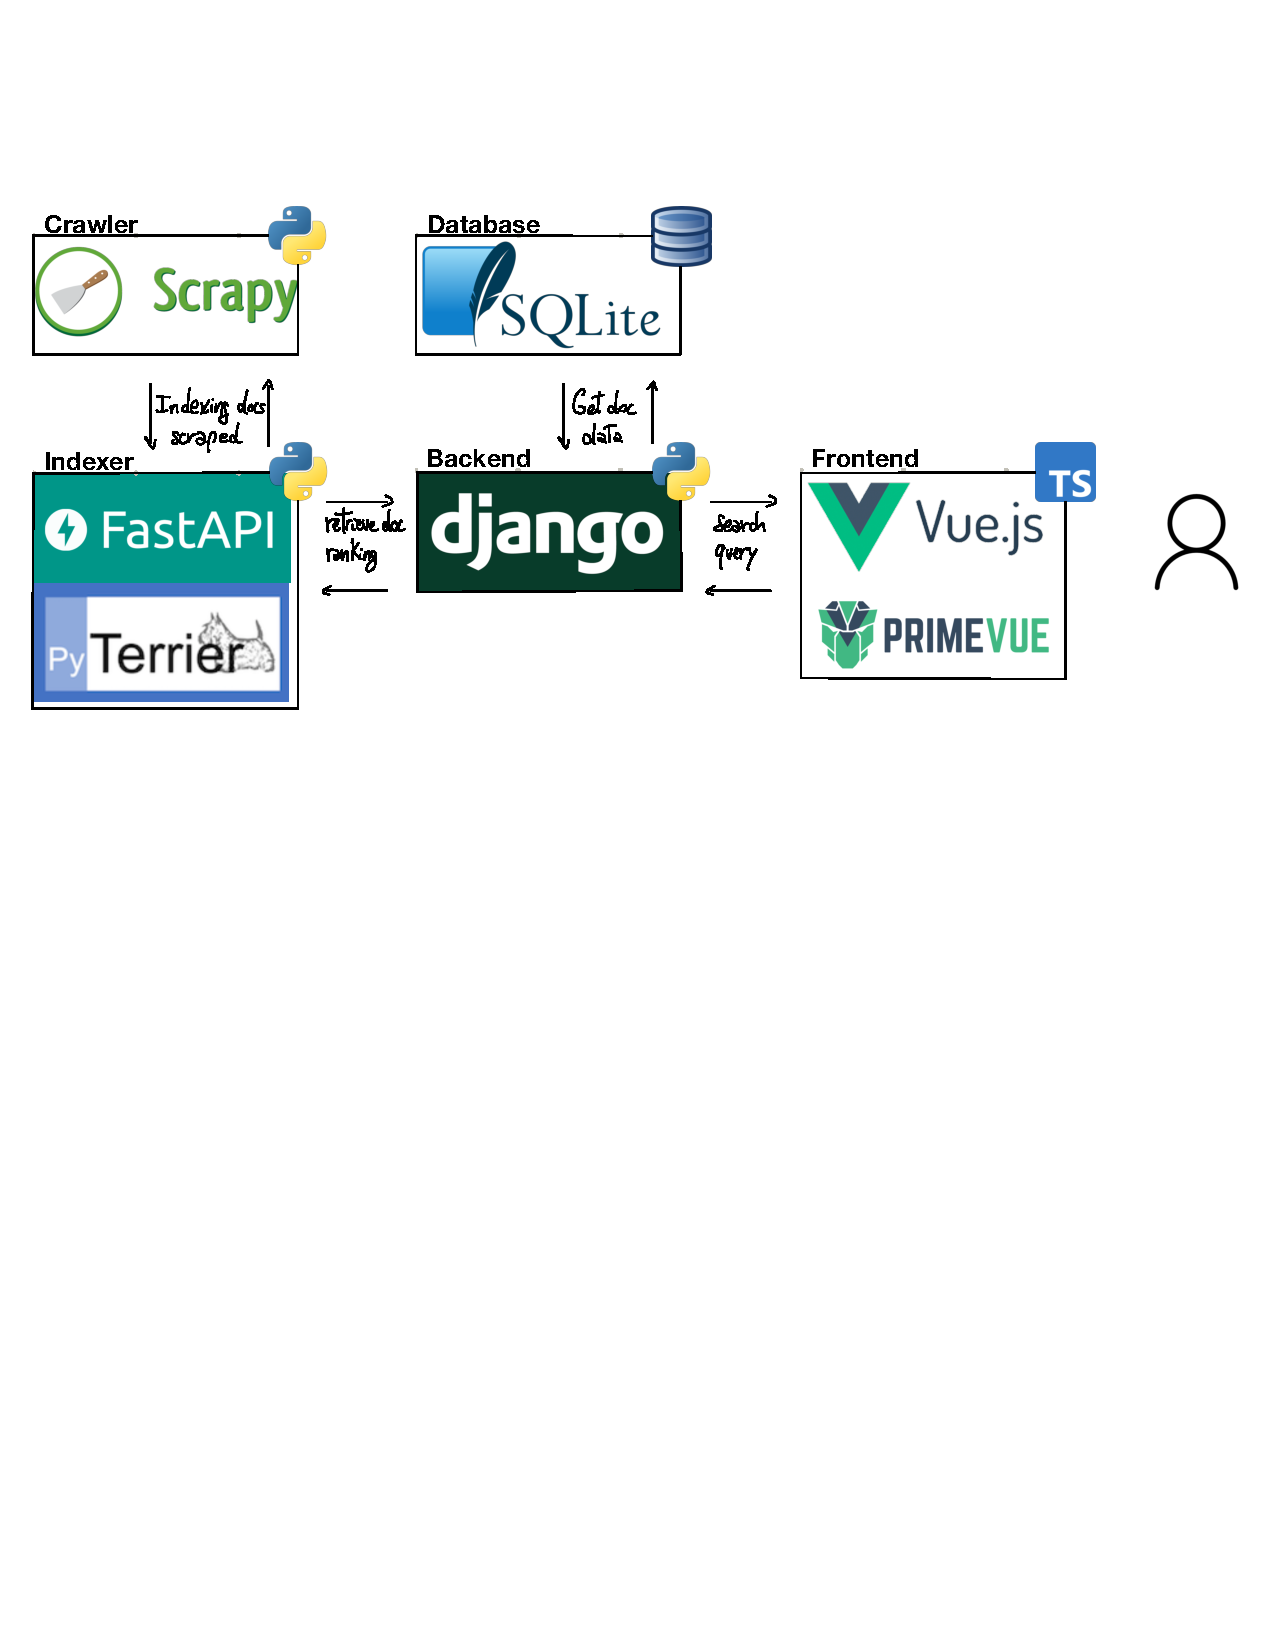
\includegraphics[width=\textwidth, trim={0cm 16cm 0cm  3cm}]{figures/architecture.pdf}
    \end{figure}


    \newpage
    \textbf{browser traces} collected in cookies for every search query user issues, part of recommender system.

    \subsection{Technology Stack}

    \subsubsection{Scrapy}
    Scrapy, a Python framework for web crawling and scraping, is utilized in to initiate the crawling/scraping process for a specified set of artworks. The extracted data is subsequently channeled into a .json file.

    \subsubsection{PyTerrier}
    PyTerrier is a Python library that provides a high-level interface for the Terrier information retrieval system. In the provided code snippet, PyTerrier is used for building an information retrieval system to search and index documents.\newline
    Our index.py file uses PyTerrier to create the index starting from the .json file

    \subsubsection{Django \& SQLite}
    The main part of the project has been carried using a Django based backend. The backend handles the main fetches from the frontend.
    The backend is also the joint between the frontend and the index, making calls to a FASTApi that returns relevant documents given a query.\newline
    To return to the frontend the main information about the documents, the backend iterates through a database in SQLite that contains the main information for each artwork

    \subsubsection{Vue.js \& PrimeVue}
    Finally, to develop the frontend, it has been used Vue.js, using the PrimeVue as UI library. Vue.js allows us to create a reactive and dynamic user interface, while PrimeVue provides us with a set of pre-built components and styles.

    %%%%%%%%%%%%%%%%%%%%%%%%%%%%%%%%%%%%%%%%%%%%%%%%%%%%%%%%%%%%%%%%%
    \section{Crawling}\label{sec:crawling}
    Harnesing (relatively) Bit Text Data characterized with the 5
    Vs \footnote{Volume, Variety, Velocity, Value, Veracity},
    we lack automating the Velocity attribute since we need to rerun the spiders manually to update its
    status on the inverted index.
    Crawling parses text that is unstructed to group them in well-structured documents, allowing them to be
    easily indexed.

    \section{Indexing}\label{sec:indexing}
    The Pyterrier platform supports indexing and retrieval operations by employing shallow
    NLP \footnote{Natural Language Processing}
    techniques to enable computers to understand the meaning of natural language text.

    \section{Retrieval}
    \subsection{Backend}
    The backend relies on a SQLite database to store the main information about the documents, making possible to retrieve the relevant ones following a call to the index.\newline
    Django serves as the foundational framework for constructing the primary structure, bringing with it a multitude of advantages such as rapid development, a robust and secure architecture, built-in administrative features, and a thriving community support ecosystem.\newline
    The backend handles the two main fetches of the application:
    \begin{itemize}
        \item /api/documents/get-documents/"query"/: This endpoint facilitates the retrieval of relevant documents based on a provided query string.
        \item /api/recommendation/get-recommended/: This endpoint is tasked with retrieving recommended artworks. By inputting a set of tags, it conducts a search within the index, returning all pertinent documents associated with the specified criteria.
    \end{itemize}

    %%%%%%%%%%%%%%%%%%%%%%%%%%%%%%%%%%%%%%%%%%%%%%%%%%%%%%%%%%%%%%%%%
    \subsection{Frontend}
    The frontend is the main part of the application, where all the features are implemented.\newline
    For the interface, it has been chosen a simple layout, consisting of only a search-bar and a search button. Once the user performs the search, the aspect of the page changes, adding new components. We will examine each of them:
    \begin{itemize}
        \item First, under the search-bar will appear a new set of control to filter the obtained results according to four main characteristics: site of origin, minimum price, maximum price and tag.
        \item Second, there will be shown some carousels for the recommended results based on the most frequents tags of the resulted artworks. Essentially, once all the artworks related to the query have been retrieved, the frontend extracts from all these artworks the related tags, it chooses the ones with the higher frequency and, using the /api/recommendation/get-recommended/ fetch, it shows a maximum of 5 results related to each tag in a moving carousel
        \item Finally, the artworks retrieved from the query are displayed in a card-like style, showing an insight of the artwork, the author, the title, the price, a short description and the main tags, with a Visit button that will bring the user to the page of that artwork in the original site
    \end{itemize}

    \subsubsection{User Interface}\label{sec:ui}

    Emotional design: key in Apple, Google alike

    Jacobs heuristics respected

    standard filtering system


    %%%%%%%%%%%%%%%%%%%%%%%%%%%%%%%%%%%%%%%%%%%%%%%%%%%%%%%%%%%%%%%%%
    \section{Evaluation}
    System evaluation: Recall and precision paragraph

    \subsection{User Evaluation}

    SUS includes pia, quote are designers users too?

    \subsubsection{User Experience}\label{sec:ux}
    Sentiment analysis


    %%%%%%%%%%%%%%%%%%%%%%%%%%%%%%%%%%%%%%%%%%%%%%%%%%%%%%%%%%%%%%%%%
    %\section{Running information}
    \section{Limitations and Future Improvements}

    The project is a \textit{Text Retrieval} system at its current state.
    Since the type of data provided by artworks is not descriptive nor verbose,
    implementing \textit{Text Analysis} features becomes troublesome because lacking the large amounts of
    text data in order to discover interesting patterns buried in text.
    Nevertheless, \textit{Text Organization} implementation feasibility is high due to
    short well-structured categorized-based descriptions usually artwork documents have,
    allowing to connect and navigate scattered information.

    %%%%%%%%%%%%%%%%%%%%%%%%%%%%%%%%%%%%%%%%%%%%%%%%%%%%%%%%%%%%%%%%%
    \section{Conclusions}
    We had fun with deciding the technology stack to use and the architecture structure.
    We enjoyed the project freedom that allowed us to put in practice all the metholodogies
    learnt from this course and all the others we had during the bachelor.

    \section{References}
    \begin{itemize}
        \item \textit{ArtForSale} GitHub project public repository:\\
              \url{https://github.com/JekxDevil/IR-ArtForSale}
    \end{itemize}

\end{spacing}
\end{document}